\section{Thu, Nov 1, 2018}

I didn't lose my faith. I lost belief in a corporate entity. I still have a belief in
God and in His Son Jesus Christ. The Holy Ghost is there to prompt things which are
true and false and to testify of the Father and the Son. No problem there at all.

Here's the problem.

The Church of Jesus Christ of Latter-day Saints. That's the problem. They claim sole
authority on everything religious. That is where I draw the line. To indicate that
every other church is false and wrong, to indicate that no matter what if you don't
become Mormon, you don't get to be with God? You can't tell me that's not what they
teach. That is exactly what they teach. How else do people get to the Celestial
Kingdom? The exact wording is:

\begin{displayquote}
Your endowment is, to receive all those ordinances in the House of the
Lord, which are necessary for you, after you have departed this life, to enable you 
to walk back to the presence of the Father, passing the angels who stand as 
sentinels, being enabled to give them the key words, the signs and tokens, 
pertaining to the Holy Priesthood, and gain your eternal exaltation in spite of 
earth and hell.\footnote{Journal of Discourses 2:31}
\end{displayquote}

Exaltation is to be with God. Mormons believe that being with God means to be in the
Celstial Kingdom, the very top level. To be under a Celestial covenant of Eternal
Marriage.\footnote{D\&C 132} The other kingdoms will not have the privlidge of being
with God and are considered hell to that person. Yet when we get to the other side,
and judgement day is upon us. We will go to that kingdom where we belong, that
kingdom which we will feel comfortable in the most. If that is the Telestial Kingdom?
So be it. If it's the Terrestial Kingdom? Yep, that works too. I imagine a very few
portion will be in Outer Darkness, well aside from Satan and those angels which
followed him before the world was. But those who gained a body, those people would
have to deny the Holy Ghost.

\begin{figure}[h!]
  \centering
  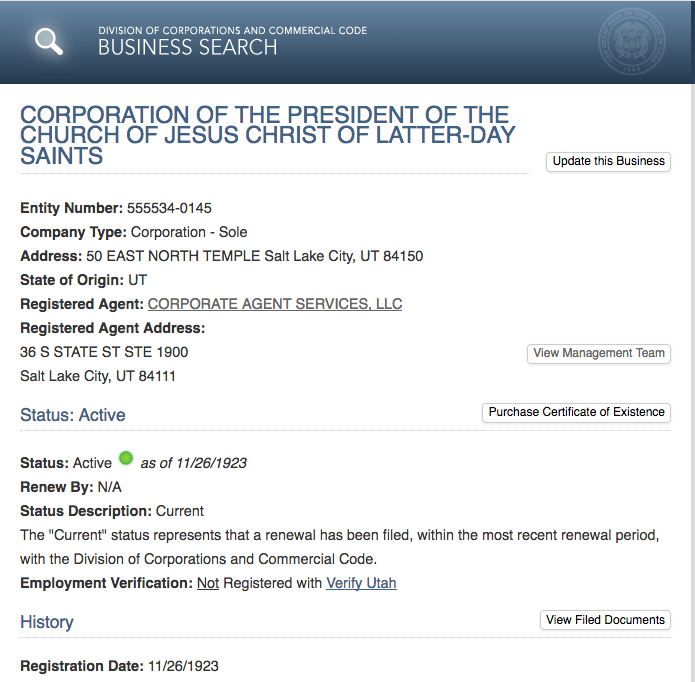
\includegraphics[width=1\linewidth]{articles/images/business.png}
  \caption{LDS Church Business Listing}
  \label{fig:business}
\end{figure}

That's what the church is. It's a business. A corporation. Why would a religious
institution need to register as a corporation? Is that simply bending to man's laws?
Why would God need to bend to man's laws? It brings about some ... interesting
questions. Polygamy, in order for Utah to become a state polygamy had to be
renounced. No longer practiced. Did God really put an end to polygamy? Or did the
people who wanted Utah to become a state put an end to polygamy?

Who really speaks for God? Recently, President Russel M. Nelson's wife, Wendy Nelson
stated the following:

\begin{displayquote}
``I have seen him changing in the last ten months," said Sister Nelson. ``It is as 
though he's been unleashed. He's free to finally do what he came to earth to do. ... 
And also, he's free to follow through with things he's been concerned about but 
could never do. Now that he's president of [the Church], he can do those
things."\footnote{Latter-day Saint Prophet, Wife and Apostle Share Insights 
of Global Ministry, Mormonnewsroom.org Article}
\end{displayquote}

That doesn't sound much like he's been receiving revelation from God regarding some
things that have to do with the church. For example, in 1990, Nelson gave a talk
about the church and how Mormon shouldn't be used. It sounds and feels like President
Nelson has had some things on his mind over the years and now that he's president of
the church, he can finally act on those thoughts. Again it goes back to how long has
Jesus been mad that the term Mormon has been used and it's been a major victory for
Satan.